% Schematic frustum-like polyhedron; no metric proportions inferred.
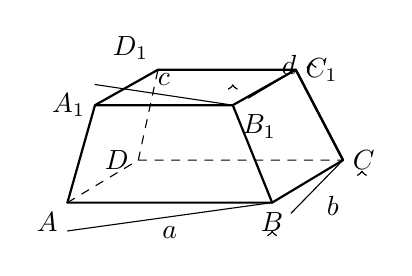
\begin{tikzpicture}[x=1cm,y=.75cm,line cap=round,line join=round]
  \coordinate (A) at (0,0);\coordinate (B) at (2.6,0);\coordinate (C) at (3.5,.72);\coordinate (D) at (.9,.72);
  \coordinate (A1) at (.35,1.65);\coordinate (B1) at (2.1,1.65);\coordinate (C1) at (2.9,2.25);\coordinate (D1) at (1.15,2.25);
  \draw[thick] (A)--(B)--(C)--(C1)--(B1)--(A1)--(D1)--(C1);
  \draw[thick] (A)--(A1) (B)--(B1) (C)--(C1);
  \draw[dashed] (A)--(D) (D)--(C) (D)--(D1);
  \draw[dashed] (D1)--(A1);
  \draw[<->] (A)++(0,-.48)--node[below] {$a$} (B)++(0,-.48);
  \draw[<->] (B)++(.24,-.18)--node[below right] {$b$} (C)++(.24,-.18);
  \draw[<->] (A1)++(0,.35)--node[above] {$c$} (B1)++(0,.35);
  \draw[<->] (B1)++(.2,.12)--node[above right] {$d$} (C1)++(.2,.12);
  \node[below left] at (A) {$A$};\node[below] at (B) {$B$};\node[right] at (C) {$C$};\node[left] at (D) {$D$};
  \node[left] at (A1) {$A_1$};\node[below right] at (B1) {$B_1$};\node[right] at (C1) {$C_1$};\node[above left] at (D1) {$D_1$};
\end{tikzpicture}
